
\documentclass[letterpaper]{article}
\usepackage[letterpaper,margin=1.75in,noheadfoot]{geometry}
\usepackage{color, enumerate, sectsty}
\usepackage[normalem]{ulem}
\usepackage{amsmath}
\usepackage{graphicx}
\graphicspath{ {Figures/} }

\newcommand{\reporttitle}{Implementation of Perceptron Algorithm}
\newcommand{\name}{Shiva Bhusal}
\newcommand{\course}{CS 6200}

\usepackage[bookmarks, colorlinks, breaklinks,
pdftitle={\name - \reporttitle},pdfauthor={\name}, unicode]{hyperref}
\hypersetup{linkcolor=magneta,citecolor=magenta,filecolor=magenta,urlcolor=[named]{WildStrawberry}}

%%% Start of our document 

\begin{document}
\begin{center}{\huge \scshape \reporttitle}\end{center}
\begin{center}\vspace{0.2em} {\Large \name\\}
  {\course}\end{center}
  
%%% Let's add sections here. 
  
  \section{Introduction}
  In this report, the experimental results of the percentron implementation has been presented. The results have been based on two different cases: 1. When all the datasets are linearly separable, and 2. When one of the datasets is not linearly separable. The Appendix section shows the demo screenshots of the implementation performed. 

  \section {Experimental Results}
  \subsection {DataSet generation}
  Dataset was generated by using a simple algorithm by gradually increasing the value of x,y,z with reference to the center of the sphere. This simple algorithm makes sure that all the points lie within the sphere of radius 2. 30 such datasets were created and passed as [4*30] dimensional array to the training method. The training method takes only first 15 datasets of the array and the classifier is trained. The rest of the datasets are used to test the accuracy of the classifier. 

  The attached screenshot in the Appendix section shows the demo result of dataset generation. 
  
  Similarly, datasets were also generated for the class B and Class C, and training is done seperately for each of the classes. 

  The three centers of spheres are (0,50,-50),(-50,-50,-50), and (50,50,50) respectively. 

  The learning rate has been set as 0.5 and threshhold has been set as 0. 

  \begin{tabular}{ |p{5cm}|p{3cm}|p{3cm}| }
 \hline
 \multicolumn{3}{|c|}{Training Datset for 3 classes} \\
 \hline
Class A& Class B & Class C\\
 \hline
0.4 50 -50 & -49.6 -50 -50 & 50.4 50 50 \\
-0.4 50 -50 & -50.4 -50 -50 & 49.6 50 50 \\
0.8 50 -50 & -49.2 -50 -50 & 50.8 50 50 \\
-0.8 50 -50 & -50.8 -50 -50 & 49.2 50 50 \\
1.2 50 -50 & -48.8 -50 -50 & 51.2 50 50 \\
-1.2 50 -50 & -51.2 -50 -50 & 48.8 50 50 \\
1.6 50 -50 & -48.4 -50 -50 & 51.6 50 50 \\
-1.6 50 -50 & -51.6 -50 -50 & 48.4 50 50 \\
2 50 -50 & -48 -50 -50 & 52 50 50 \\
-2 50 -50 & -52 -50 -50 & 48 50 50 \\
0 50.4 -50 & -50 -49.6 -50 & 50 50.4 50 \\
0 49.6 -50 & -50 -50.4 -50 & 50 49.6 50 \\
0 50.8 -50 & -50 -49.2 -50 & 50 50.8 50 \\
0 49.2 -50 & -50 -50.8 -50 & 50 49.2 50 \\
0 51.2 -50 & -50 -48.8 -50 & 50 51.2 50 \\

 \hline

\end {tabular}

  \subsection {Case 1: All the dataSets are linearly seperable}
  After the training was succesful, next 15 datasets were used for testing the classifier. The sample test result looked like this for the second half of the class A dataSets. Similar process was repeated for the second half of class B and class C datasets. The output of the execution is presented in the table below: 


 \begin{tabular}{ |p{5cm}||p{5cm}| }
 \hline
 \multicolumn{2}{|c|}{Testing Result for second half of Class A dataset} \\
 \hline
Data Points& Class\\
 \hline
0,48.8,-50 & Class A \\
0,51.6,-50 & Class A \\
0,48.4,-50 & Class A \\
0,52,-50 & Class A \\
0,48,-50 & Class A \\
0,50,-49.6 & Class A \\
0,50,-50.4 & Class A \\
0,50,-49.2 & Class A \\
0,50,-50.8 & Class A \\
0,50,-48.8 & Class A \\
0,50,-51.2 & Class A \\
0,50,-48.4 & Class A \\
0,50,-51.6 & Class A \\
0,50,-48 & Class A \\
0,50,-52 & Class A \\
 
 \hline

\end {tabular}

 \begin{tabular}{ |p{5cm}||p{5cm}| }
 \hline
 \multicolumn{2}{|c|}{Testing Result for second half of Class B dataset} \\
 \hline
Data Points& Class\\
 \hline
-50,-51.2,-50 & Class B \\
-50,-48.4,-50 & Class B \\
-50,-51.6,-50 & Class B \\
-50,-48,-50 & Class B \\
-50,-52,-50 & Class B \\
-50,-50,-49.6 & Class B \\
-50,-50,-50.4 & Class B \\
-50,-50,-49.2 & Class B \\
-50,-50,-50.8 & Class B \\
-50,-50,-48.8 & Class B \\
-50,-50,-51.2 & Class B \\
-50,-50,-48.4 & Class B \\
-50,-50,-51.6 & Class B \\
-50,-50,-48 & Class B \\
-50,-50,-52 & Class B \\
 \hline

\end {tabular}

\begin{tabular}{ |p{5cm}||p{5cm}| }
 \hline
 \multicolumn{2}{|c|}{Testing Result for second half of Class C dataset} \\
 \hline
Data Points& Class\\
 \hline
50,48.8,50 & Class C \\
50,51.6,50 & Class C \\
50,48.4,50 & Class C \\
50,52,50 & Class C \\
50,48,50 & Class C \\
50,50,50.4 & Class C \\
50,50,49.6 & Class C \\
50,50,50.8 & Class C \\
50,50,49.2 & Class C \\
50,50,51.2 & Class C \\
50,50,48.8 & Class C \\
50,50,51.6 & Class C \\
50,50,48.4 & Class C \\
50,50,52 & Class C \\
50,50,48 & Class C \\
 \hline

\end {tabular} \\

Accuracy=(No of correct classifications)/ Total dataSets =100 percent 


\subsection {Case 2: One of the Datasets is not linearly separable}
In this case, the 15th and the 30th dataset of each of the classes have been changed to make sure that the point is linearly inseparable. 

  \begin{tabular}{ |p{5cm}||p{5cm}| }
 \hline
 \multicolumn{2}{|c|}{Result for 2nd Half of class A datasets} \\
 \hline
Data Points& Class\\
 \hline
0,48.8,-50 & Class A \\
0,51.6,-50 & Class A \\
0,48.4,-50 &  Class A \\
0,52,-50 &  Class A  \\
0,48,-50 &  Class A \\
0,50,-49.6 &  Class A \\
0,50,-50.4 &   Class A \\
0,50,-49.2 &  Class A \\
0,50,-50.8 &  Class A \\
0,50,-48.8 &  Class A \\
0,50,-51.2 &  Class A \\
0,50,-48.4 &  Class A \\
0,50,-51.6 &  Class A \\
0,50,-48 &  Class A \\
90,90,100 &  Class A \\
 
 \hline


\end{tabular}

 \begin{tabular}{ |p{5cm}||p{5cm}| }
 \hline
 \multicolumn{2}{|c|}{Result for 2nd Half of class B datasets} \\
 \hline
Data Points& Class\\
 \hline
-50,-51.2,-50 & Class C \\
-50,-48.4,-50 & Class C \\
-50,-51.6,-50 & Class C \\
-50,-48,-50 & Class C \\
-50,-52,-50 & Class C \\
-50,-50,-49.6 & Class C \\
-50,-50,-50.4 & Class C \\
-50,-50,-49.2 & Class C \\
-50,-50,-50.8 & Class C \\
-50,-50,-48.8 & Class C \\
-50,-50,-51.2 & Class C \\
-50,-50,-48.4 & Class C \\
-50,-50,-51.6 & Class C \\
-50,-50,-48 & Class C \\
101,101,101 & Class A \\
 \hline
\end{tabular} \\

\begin{tabular}{ |p{5cm}||p{5cm}| }
 \hline
 \multicolumn{2}{|c|}{Result for 2nd Half of class C datasets} \\
 \hline
Data Points& Class\\
 \hline
50,48.8,50 & Class A \\
50,51.6,50 & Class A \\
50,48.4,50 & Class A \\
50,52,50 & Class A \\
50,48,50 & Class A \\
50,50,50.4 & Class A \\
50,50,49.6 & Class A \\
50,50,50.8 & Class A \\
50,50,49.2 & Class A \\
50,50,51.2 & Class A \\
50,50,48.8 & Class A \\
50,50,51.6 & Class A \\
50,50,48.4 & Class A \\
50,50,52 & Class A \\
-70,-70,-70 & Class C \\ 
 
 \hline
\end{tabular} \\

Accuracy=No of correct classifications/ Total dataSets =16/45=35.5 percent 

\section {Summary}
  In part 1 where all the points were linearly separable, the model was 100 percent accurate for all the given test dataSet whereas in part 2 where 1 point was linearly inseparable in the training Set, the model gave suprising results with just 35 percent accuracy. The changes in the learning rate changes the no of iterations it takes to converse into the correct values of the weights. 
  
\section {Appendix}

\begin{figure}[h]
\caption{Initial Build and Run}
\centering
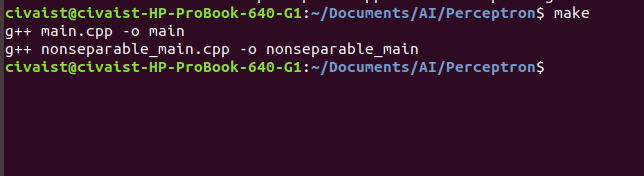
\includegraphics[width=10cm,height=8cm]{make}
\end{figure}

\begin{figure}[h]
\caption{Dataset generation for the given center of spheres}
\centering
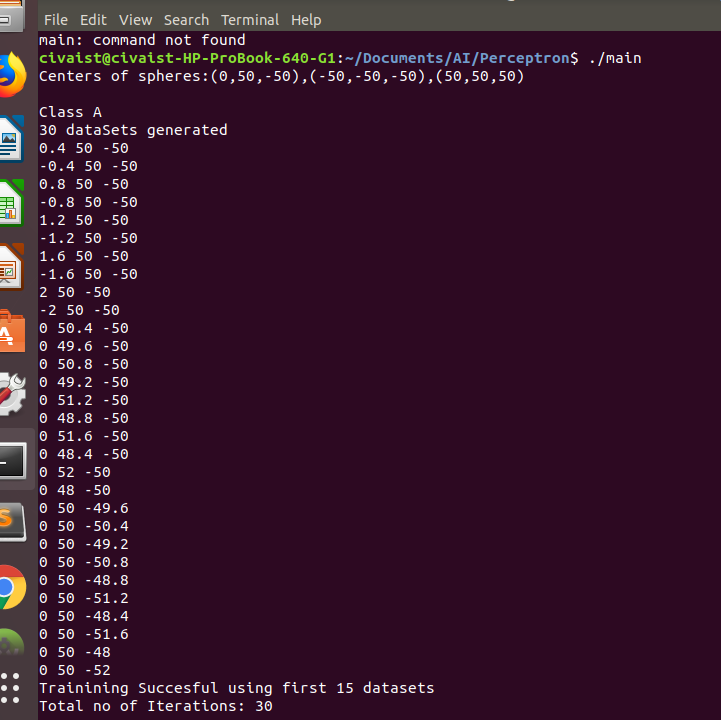
\includegraphics[width=10cm,height=8cm]{Dataset_generation}
\end{figure}

\begin{figure}[h]
\caption{Sample Test Result}
\centering
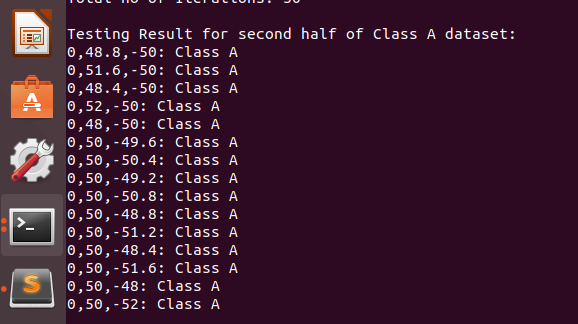
\includegraphics[width=10cm,height=8cm]{test_result}
\end{figure}
 
\end{document}

%%% End of our document 
